\chapter{Introduction}
\graphicspath{ {chapters/Introduction/} }

Nowadays in the manufacturing industry most of the production is automated. This is being referred to as the Industry 3.0 or the third industrial revolution. \\ 

\begin{figure}[h]
	\caption{Industry 4.0 \cite{pictIndustry40}}
	\centering
	  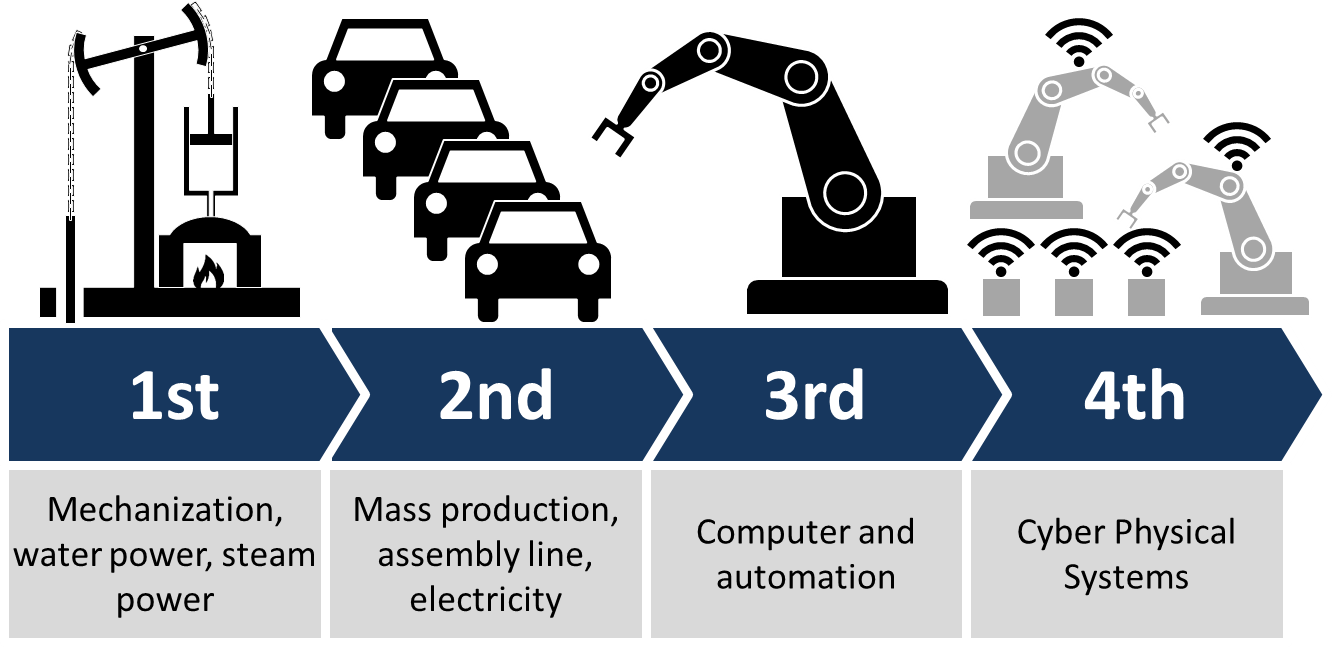
\includegraphics[width=1\textwidth]{industry-40.png}
\end{figure}

	
 Parts of the product are created and assembled in robotic cells or robotic assembly lines. When developing a new product the engineers usually create a CAD model of the product and based on that build prototypes. When refined a different engineering team is tasked with designing an assembly line that could mass produce the parts and assemble them together. \\
 
It widely is believed that the future (Industry 4.0) will revolve around automation and data exchange. These so called \"smart factories\" should be able to manufacture goods with unprecedented effectivity and ease. Beyond Industry 4.0, smart factories will only reach their potential when we'll be able to design a product and then just let a factory manufacture it for us without human intervention.   

Currently, assembly lines are designed in a specific type of CAD software, which allows the simulation of the full assembly sequence. This way the engineers can validate the reachability and collision clearance of the prepared line, including human factors. One example of such software is the Tecnomatix suite by SIEMENS. Tecnomatix Process Simulate is an industry leading software for digital manufacturing, used by the likes of Volkswagen or Samsung \cite{TecnomatixCustomers}. \\ 

When designing an assembly line for a product the focus is on the successful creation of the product, which in itself is a no mean feat. Then searching for the optimal layout of the robots and schedule of the tasks that need to be executed for the desired result is an inhuman task. 

\section{Motivation}

Rather than focusing the question of the layout of the robots which would require knowing the available space, layout of the factory, location of the power outlets and so on. Since this problem would be bigger than one lifetime of work, we need to apply the divide and conquer principle. Rather than looking at the whole problem this thesis tries to tackle a smaller part, hoping that other research could build on it. The goal is to take the human design of the assembly line and apply a mathematical model to find the optimal schedule which could be used to marginally improve the effectivity of the line. \\

The schedule can be optimized with various goals in mind. Traditionally this has been cycle time, allowing the factories to increase their output marginally, however the recent trend is to look at energy usage as well, or in some cases primarily energy usage.\\

Optimizing energy usage even a small improvement could have enormous impact on the yearly savings. For example in the case of General Motors their factories drew about 9 terawatt hours in 2015 \cite{GMEnergySpending}. According to Meike et al. \cite{Meike8Percent} about 8\% of the energy used in the factories is consumed by industrial robots. Assuming consumer pricing of 10 cents per kWh even with 1 percent improvements in energy efficiency this roughly equates to \$~720000 in potential savings. In addition to that the manufacturing business is also affected by government regulations such as the plan of the European Union for energy savings \cite{EUElectricity}.

\section{Related Work}

Of course the optimization of robotic cells, due to the outstanding potential improvements, is nothing new. Due to its raw scale the optimization is mostly pronounced in the automotive industry, however the concepts translate to all different kinds of fields. As shown by R.G. Fenton et al. \cite{OptimizationCycleTimeFenton} a position of the robots in a multi-location industrial work-cell can have profound effect on the cycle time. An optimal position  can be determined through the use of a numerical optimization routine and a kinematic computer graphics simulation program. \\

Another approach at optimizing the effectiveness of robotic cells was shown by Jiafan Zhang et al. \cite{OptimizationCycleTimeZhang}. To achieve improvements in cycle time his group focused mainly at the grippers, which are an essential part of many robotic cells. In this paper, an analytical framework for scheduling moving of robot with single- or dual-gripper is developed. Initially they consider different constraints in validation, including interval/free pick up, non-free/free process, and inadmissible path. The paper indicates that a dual-gripper robot can gain an improvement in throughput in most cases. \\

Recently Edvin Åblad et al. \cite{CollisionAvoidanceAblad} took a look at the practical challenges of real assembly line designs. An area that caught their eye with the most room for improvement was the way collisions are usually treated. Collisions are avoided by introducing synchronization schemes among the robots, preventing shared volumes of the workspaces to be simultaneously entered. Synchronization often increases the cycle time and makes the robot programming more difficult to generate, adjust, and maintain. In this paper, they present a novel method to maximize throughput while eliminating all synchronizations among robots. \\

!!!
Davis Meike et al. \cite{Meike8Percent}
This paper quantitatively reports about potential energy savings on robotic assembly lines for the automotive industry. At first, a detailed system model is described, which improves previously published results by explicitly considering both manipulator and electrical drive dynamics. The model closely captures experimental data in terms of actuation torques and servo-drive voltages, which are directly used to derive the plant input power. Two practical methods are then evaluated for reducing the overall energy consumption. The methods rely on: 1) implementation of energy-optimal trajectories obtained by means of time scaling, concerning the robots' motion from the last process point to the home positions and 2) reduction of energy consumption by releasing the actuator brakes earlier when the robots are kept stationary. Simulation results, based on the production timing characteristics measured at a real plant, clearly shows that the system energy consumption can be effectively reduced without negative effects on the production rate. \\
!!!
+top 3 z references
!!!

This study by L. Bukata et al. \cite{EnergyOptimisationBukata} focuses on the energy optimization of industrial robotic cells. They have devised a mathematical model, which takes into account various robot speeds, positions, power-saving modes, and alternative orders of operations. This model can be transformed into a mixed-integer linear programming formulation. Due to speed concerns they also created a hybrid heuristic capable of utilizing multi-core processors. Experiments show that theoretically, the energy consumption can be reduced by as much as 20\% merely by optimizing the robot speeds and applying power-saving modes. \\

From the selection of practical works the most interesting is research done by Anne-Laure Coiffier \cite{AnneBacktracking}, which also focuses on the Tecnomatix suite of tools. The goal of her work was to find a valid schedule for a given setup of robotic cells and robotic actions with fixed duration. The algorithm performs a mapping of the tasks to the given resources, taking into account the material flow. For this a Depth-First Search algorithm with backtracking is used. \\

In comparison to Anne's work we want to 

There are multiple articles regarding the optimization algorithms used. For this reason I chose to make this work focus on the practical part of connecting the optimization algorithm and the tool itself.


strukturovaneww co se tyce algoritmu, toolu, atd\ldots vypichnuti thedulezitych veci co vyuzije sekce Contribution)

\section{Contribution and Outline}

One thing all of the works above have in common is the lack of a practical application. Mathematical models are devised, algorithms are implemented, however the works don't offer full integration with the world assembly line design where the proposed improvements could be leveraged. Closes to this came the work from Anne... 

vzhledem k existujicim pracem neexistuje takova a takova prace + popis inovaci, a v pristi sekci bude ... a pak ... atd ...

This work could bridge the world of theoretical improvements and algorithms with the practical world.; 

The schedule could be optimized with different goals in mind, for example: cycle time or energy consumption (leveraging the robots sleep modes). This work focuses on building the bridge between the design tool and a MILP model which can be swapped out. \\


outline duh

\section{Problem Statement}

In the assembly line we consider robots as the main actor. Humans can be also counted as a robot for the optimization purposes. Every robot as a set of actions that he needs to perform, and the action can also depend on other action. 
- Mejme n robotu a mejme graf co popisuje operace\ldots 
